\section{Introduction}
\label{sec:usbe_lung_introduction}
\subsection{A review of previous work on diagnostic ultrasound-induced lung hemorrhage}
\label{subsec:usbe_lung_bio_intro}
\ac{DUS} is the safest form of medical imaging available today and has
become ubiquitous in clinical practice. Currently, the only known
bioeffect of non-contrast \ac{DUS} known to occur in mammals is
\ac{LH}. The physical damage mechanisms underlying, \ac{DUS}-induced
\ac{LH} are presently unknown, though the damage does not appear to be
particularly severe, and is not considered a problem of significant
clinical concern. However, it is an important problem to understand if
we hope to improve lung \ac{DUS} by expanding the US regimes used in
clinical application. In this work, we use numerical experiments to
investigate the underlying physics of \ac{DUS} wave-lung
interaction. We model the lung as a compressible multi-fluid system
and solve the Euler equations of inviscid fluid motion to study the
dynamics of fluid-fluid interfaces exposed to acoustic waves relevant
to \ac{DUS}. We observe that acoustically-generated vorticity at
perturbed water-air interfaces drives the interface to deform. We
hypothesize that a similar mechanism may be responsible for deforming
and ultimately rupturing the fragile tissue barriers around alveoli,
tiny air sacs within the lungs, leading to \ac{DUS} induced \ac{LH}.

\ac{US}-induced \ac{LH} is not a new problem. It was first discovered
in mice over 20 year ago \citep{Child1990}. Since then, the use of
lung \ac{DUS} has become increasingly common in certain critical care
situations \citep{Lichtenstein2009}. And there has been much work to
better understand the problem of \ac{DUS}-induced \ac{LH}. Previous
research has primarily aimed at three specific ends: (1) Determining
the dependence of damage characteristics and thresholds on the
characteristics of the \ac{US} subject; (2) Determining the dependence
of damage characteristics and thresholds on the \ac{US} properties;
and (3) Investigating the physical damage mechanism causing the
hemorrhage.  Our work aims to contribute to this third area by
investigating the fundamental physics underlying the problem.

Work in the first area has considered species, age, physiological
development, and pulmonary state of the \ac{US} subject as possible
variables which \ac{DUS}-induced \ac{LH} may depend upon.  Within
mammals, \ac{DUS}-induced \ac{LH} has been observed to be largely
species indiscriminate and has been found to occur in mice, pigs,
rats, rabbits, and monkeys \citep{Baggs1996, Child1990, Dalecki1997,
  Frizzell1994, Frizzell2003, Harrison1995, Holland1996, Kramer2001,
  OBrien1997a, OBrien2001b, OBrien2003a, OBrien2005, OBrien2000,
  OBrien2001a, Penney1993a, Raeman1993, Raeman1996, Tarantal1994a,
  Zachary1995a, Zachary2001, Zachary2001a}. \cite{Dalecki1997}
investigated the effect of age on \ac{DUS}-induced \ac{LH} in mice by
exposing neonatal, juvenile, and adult mice to \ac{DUS} pulses. The
study found that while hemorrhage thresholds were similar in all mice,
the degree of hemorrhage was much greater in the adult mice than in
the younger subjects. Similarly, \cite{OBrien2003a}, studied the age
dependence of hemorrhage in pigs, and found that older pigs had a
significantly lower hemorrhage thresholds than juvenile and
middle-aged pigs. In an unexpected result, the study also found that
if one lung was exposed to \ac{US} and the pig was then rolled over
and the second lung exposed, the hemorrhage threshold in the second
lung was substantially lower than in the first. In a separate study,
\cite{OBrien2002a} subjected rats with variable degrees of lung
inflation to \ac{DUS} in order to study the role of the impedance
boundary condition at the lung’s pleural surface on \ac{LH}. It was
found that rats with deflated lungs, that had less impedance mismatch
with their surroundings, were more easily damaged than deflated
lungs. While no direct experimentation has been performed on humans,
for obvious ethical reasons, \cite{Meltzer1998} found that
transesophageal echocardiography with similar \ac{US} parameters to
those causing lung hemorrhage did not lead to visible hemorrhage on
the surface of the lung. While \ac{DUS}-induced \ac{LH} has not been
shown to occur in humans, it has been demonstrated in a wide variety
of mammals of varying age and size. The work presented here is not
specific to any particular species or subject, but aims to consider
the more general physical problem at hand.


The second area of research, investigating the dependence of lung
hemorrhage on \ac{US} properties, has seen the largest amount of work
and is important for designing \ac{US} in a way that is capable of
high quality diagnostic imaging while minimizing any unwanted
bioeffects. Research in this area has looked at the dependence of
hemorrhage on \ac{US} waveform and dosimetric properties.
\cite{Zachary1995a} used continuous-wave and pulsed-wave \ac{US} in
mice, rabbits, and pigs, and found that while the continuous- and
pulsed-wave-induced lesions appear macroscopically similar, they
differ microscopically.  Hemorrhage induced by continuous wave \ac{US}
consisted primarily of plasma and contained some cells, whereas
pulsed-wave induced hemorrhage was composed largely of cells and
contained little plasma. \cite{Raeman1996} subjected mice to pulsed
\ac{US} with varying exposure time and concluded that while threshold
amplitudes appeared insensitive to exposure time, suprathreshold
damage increased with increasing exposure. \cite{OBrien2001}
investigated the effects of \ac{US} beamwidth and found that as
beamwidth increased so did the incidence, surface area, and volume of
hemorrhage. It was noted that lung hemorrhage is perhaps the only
known beamwidth-dependent mechanical bioeffect of \ac{US}.
\cite{OBrien2003c} found evidence that increasing \ac{US} pulse
duration increases the likelihood of lung hemorrhage in rats. In this
effort we consider the dependence of the alveolar wall dynamics on
acoustic properties relevant to \ac{US}, including acoustic wave
amplitude, duration, and pressure gradient, which we relate back to
\ac{US} more closely in our discussion of our results (See Section
\ref{subsec:usbe_lung_further_discussion}).

While work in the third area of research, studying the cause of
\ac{DUS}-induced \ac{LH}, has not yet led to a conclusive
determination of the specific physical damage mechanisms, the most
common ultrasound bioeffects mechanisms have been shown to be unlikely
causes of the damage. \cite{Zachary2006} found that \ac{DUS}-induced
lung lesions do not appear similar to those induced by heat, and hence
concluded that thermal damage mechanisms are
unlikely. \cite{OBrien2000} observed that the severity of
\ac{DUS}-induced \ac{LH} in mice increased under raised hydrostatic
pressure. And \cite{Raeman1996} notes that hemorrhage is unaffected by
the introduction of \ac{US} contrast agents into subjects. Both of
these findings suggest that \ac{IC} is not a likely cause of
\ac{DUS}-induced \ac{LH}. However, \cite{Holland1996} reports
detecting cavitation during \ac{DUS}-lung interaction in
rats. \cite{Tjan2007,Tjan2008} model \ac{DUS} of the lung as an
inviscid, free surface subjected to a Gaussian velocity potential and
perform simulations to find that this setup can lead to the ejection
of liquid droplets. They go on to say that \ac{DUS} of the lung may
similarly lead to ejected droplets capable of puncturing the
air-filled sacs within the lung. Despite these efforts, the precise
damage mechanism underlying \ac{DUS}-induced \ac{LH} is still
unknown. In this work we propose a previously unconsidered mechanical
damage mechanism and perform simulations to investigate its
feasibility.

\subsection{A review of previous work on driven fluid-fluid interfaces}
\label{subsec:usbe_lung_fluids_intro}
Within the fluids community, there has been extensive research into
the fundamental physics describing interactions between mechanical
waves and fluid interfaces. Much of this research is motivated by
applications in fusion energy and astrophysics and accordingly has
investigated the \ac{RMI}, in which a perturbed fluid-fluid interface
is accelerated by a shock, causing the interface perturbation to grow
\citep{Brouillette2002,Drake2006}. The growth is driven by a sheet of
baroclinic vorticity deposited along the interface as a result of
misalignment between the pressure gradient across the shock and the
density gradient across the perturbed interface. This physical
mechanism by which these misaligned gradients create a torque on fluid
particles and generate vorticity can be thought of in terms of a
hydrostatic balance upon a particle. Pressure gradients result in
acceleration of the flow. This acceleration is inversely proportional
to density, resulting in shear and vorticity \cite{Heifetz2015}. This
is illustrated in Figure \ref{fig:usbe_lung_baroclinic_schematic}.
The existence of baroclinic vorticity can be shown by taking the curl
of the conservation of momentum equation for a compressible fluid,
however we note that it is a nonlinear effect cannot be explained by
traditional linear acoustics.
\ref{fig:usbe_lung_baroclinic_schematic} from \cite{Heifetz2015}.
\begin{figure}
  \centering
  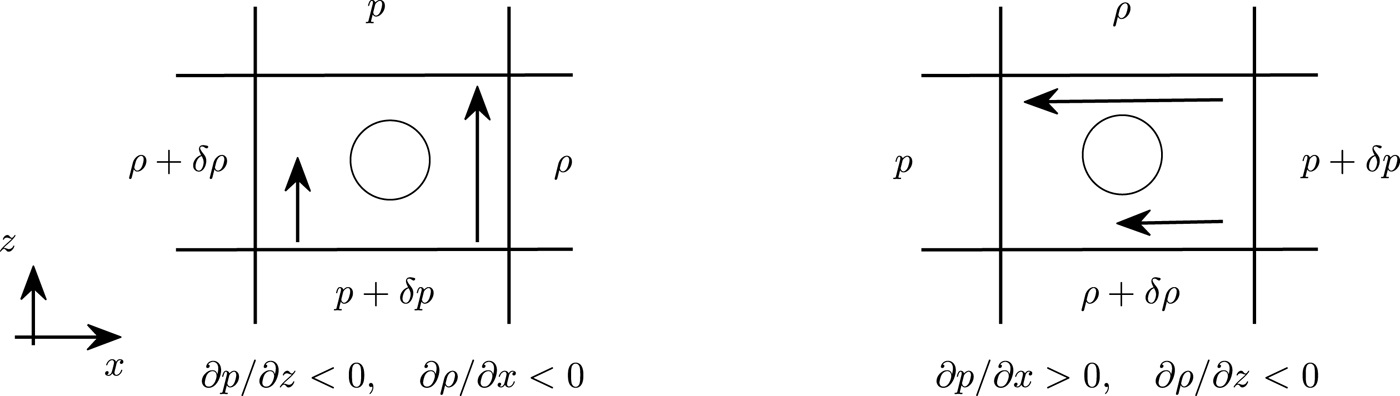
\includegraphics[width=0.9\textwidth]{./figs/lung_figs/baroclinic_schematic} \hfill
 \caption[A schematic of baroclinic torque]{From
    \cite{Heifetz2015}. A hydrostatic force balance upon a particle
    subject to perpendicular pressure and density gradients
    illustrates baroclinic torque on a fluid particle.}
  \label{fig:usbe_lung_baroclinic_schematic}
\end{figure}

For the classical \ac{RMI} setup, a planar shock impinges normally
upon the peaks and troughs of a sinusoidal interface. As the degree of
misalignment varies along the interface, the interface is accelerated
non-uniformly. The direction of the vorticity changes where the
slope of the interface changes. This counter rotation on either side
of interface peaks and troughs entrains nearby fluid causing interface
peaks to accelerate in one direction and troughs to accelerate in the
opposite direction. This results in a ``bubble'' of light fluid
penetrating the heavy fluid, and a ``spike'' of heavy fluid
penetrating the light fluid. How exactly this occurs varies slightly
depending on the relative densities of the two fluids. For the case of
a wave moving from a light fluid into a heavy one, the peaks and
troughs of the interface are initially accelerated to move away from
one another, and the interface perturbation amplitude undergoes growth
exclusively. For the case of a wave moving from a heavy fluid to a
lighter fluid, the peaks and troughs of the interface are accelerated
such that they initially move closer to one another decreasing the
perturbation amplitude. They then pass one another, inverting the
phase of the interface perturbation, and then continue moving in
opposite directions, growing the perturbation amplitude. This process
is illustrated in Figure \ref{fig:rmi_schematic}, which has been
adapted from \cite{Brouillette2002}.
\begin{figure}
  \centering
  \def\svgwidth{0.9\textwidth}
  \import{./figs/lung_figs/}{brouillette_fig3_mod.pdf_tex} \hfill%
  \caption[A schematic view of the \ac{RMI} instability for a
  heavy-light interface]{Adapted from \cite{Brouillette2002}. The
    \ac{RMI} for a heavy-light interface is illustrated. The initial
    condition (left), circulation post wave-interface interaction
    (center), and perturbation growth (right) are shown.}
  \label{fig:rmi_schematic}
\end{figure}

Previous studies of the \ac{RMI} has utilized theory, computation, and
experiments to describe the behavior of the interface after the wave
has passed. \cite{Richtmyer1960} performed the linear stability
perturbation analysis developed by \cite{Taylor1950} for the case of
an impulsive acceleration to create a model for the initial growth of
the interface perturbation. \cite{Meshkov1969} experimentally
confirmed Richtmyer's qualitative predictions, hence the name of the
instability. \cite{Meyer1972} performed numerical simulations of the
\ac{RMI} and found good agreement with Richtmyer for the case of a
shock impinging upon a light-heavy interface. \cite{Fraley1986} used
Laplace transforms in order to find the first analytical solution for
the asymptotic growth rate for a shocked interface between perfect
gases. To describe the late time, nonlinear growth of the
perturbation, \cite{Zhang1997} used single mode perturbation, keeping
many high order terms, to describe the velocity of the bubble and
spike regions of the fluid. \cite{Sadot1998} combined the linear,
impulsive solution with potential flow models of the asymptotic
behavior of the bubble and spike to develop a model for the
perturbation growth that is in good agreement with shock tube
experiments for shocks with Mach numbers Ma=1.3, 3.5. Vortex theory
has also been used to describe the behavior of the
interface. \cite{Jacobs1996} horizontally oscillated a container with
two vertically stratified liquids to obtain standing waves and then
bounced the container off of a coil spring to study the incompressible
\ac{RMI}. The late time evolution of is interface is modeled using a
row of line vorticies to obtain qualitatively similar results to those
experimentally observed, however the late-time growth rate is
underestimated. \cite{Samtaney1994} used shock polar analysis to find
the circulation deposited by a shock on planar and non-planar
interfaces. Their results are validated using and Euler code and found
to be within 10\% of the computed value for $1.0\,<\,$Ma$\,\leq\,1.32$
for all $\rho_2/\rho_1\,>\,1$, and
$5.8\,\leq\,\rho_2/\rho_1\,\leq\,32.6$ for all Ma. This work aims to
add to the current body of work on this topic by investigating
interfaces accelerated by pressure waves within the acoustic regime.

\subsection{Explanation and contributions of the present work}
\label{subsec:usbe_lung_contribution_intro}
We argue that the basic problem setup of the \ac{RMI}, a mechanical
wave impinging upon a material interface, is similar to \ac{DUS} of
the lungs. Accordingly we propose another possible damage mechanism of
\ac{DUS}-induced \ac{LH}. We hypothesize that misalignment between the
pressure gradients in the \ac{DUS} pulses and the sharp density gradients
across the    tissue-air interfaces of the lungs creates a torque around
the alveoli, which deforms and ultimately hemorrhages the alveolar
walls.

The detailed nonlinear interactions between acoustic waves and
perturbed fluid-fluid interfaces does not appear to have been
previously studied in this manner or context. This work is separate
from previous research into the \ac{RMI} as a result of the acoustic
waves being studied. Unlike shock waves, which occur over a few
molecular mean free paths and interact nearly instantaneously,
acoustic waves have a finite spacial wavelength and can occupy a much
larger portion of space. Consequently, their interaction with
interfaces occurs over a longer period of time, the duration of which
depends on a variety of factors including shape and amplitude of the
waveform, the speed of sound in the media, the relative orientation of
the traveling wave and the interface (e.g., the shape of the
interface). This duration can also be thought of in terms of the
relative sizes of the physical features of the interface and the
wavelengths of each feature of the acoustic wave of interest. Simple
\ac{RMI} analysis assumes an impulsive acceleration, and does not
apply to this work because the interface has time to deform throughout its
interaction with the wave. In this work we demonstrate that the finite
duration of the wave-interface interaction can effect the qualitative
behavior of the on interface dynamics because of the interface
deformation that occurs during this period. We will specifically
attempt to address the following questions:
\begin{enumerate} \label{itm:usbe_lung_questions}
\item Are acoustic waves capable of generating sufficient baroclinic
  vorticity at perturbed fluid-fluid interfaces for substantial
  deformations?
\item what is the impact of the acoustic wave properties, such as
  amplitude and wave duration, on the vorticity and interface
  dynamics?
\end{enumerate}

In the remainder of this work, we will first present a simplified
model problem and a set of numerical experiments designed to
investigate the fundamental physics underlying interactions between
acoustic waves and perturbed interfaces between fluids. The simulation
results and related analysis will be presented and discussed first in
the context of the fluid dynamics. We will then draw from these
results to further elaborate on the significance of these results as
they regard to the motivating problem of \ac{DUS}-induced lung
hemorrhage. We will finally end by summarizing the main conclusions
drawn from this work and suggest the next steps to be taken.

%%% Local Variables:
%%% mode: latex
%%% TeX-master: "../../prelim"
%%% End:
